\chapter{Formas de Conexionado de entradas y salidas}

\section{Salida digital}
\begin{figure}[!htp]
	\centering
	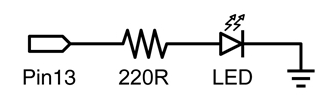
\includegraphics[width=120pt]{./Imagenes/Documentos/ArduinoNotebook_img01.png}
	\caption[Conexión Salida digital]{Conexion Salida digital}
\end{figure}

Éste es el ejemplo básico equivalente al 'hola mundo' de cualquier lenguaje de programación haciendo simplemente el encendido y apagado de un led. En este ejemplo el LED está conectado en el pin13, y se enciende y se apaga 'parpadea' cada segundo. La resistencia que se debe colocar en serie con el led en este caso puede omitirse ya que el pin13 de Arduino ya incluye en la tarjeta esta resistencia,
\begin{lstlisting}
int ledPin = 13; // LED en el pin digital 13

void setup()     // configura el pin de salida
{
   pinMode(ledPin, OUTPUT); // configura el pin 13 como salida
}

void loop()     // inicia el bucle del programa
{
   digitalWrite(ledPin, HIGH); // activa el LED
   delay(1000); // espera 1 segundo
   digitalWrite(ledPin, LOW); // desactiva el LED
   delay(1000); // espera 1 segundo
}
\end{lstlisting}
\newpage{}
\section{Entrada digital}
\begin{figure}[!htp]
	\centering
	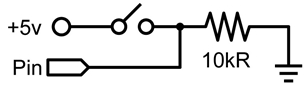
\includegraphics[width=120pt]{./Imagenes/Documentos/ArduinoNotebook_img02.png}
	\caption[Conexión Entrada digital]{Conexión Entrada digital}
\end{figure}

Ésta es la forma más sencilla de entrada con sólo dos posibles estados: encendido o apagado. En este ejemplo se lee un simple switch o pulsador conectado a PIN2. Cuando el interruptor está cerrado en el pin de entrada se lee ALTO y encenderá un LED colocado en el PIN13:
\begin{lstlisting}
int ledPin = 13; // pin 13 asignado para el LED de salida
int inPin = 2; // pin 2 asignado para el pulsador

void setup() // Configura entradas y salidas
{
   pinMode(ledPin, OUTPUT); // declara LED como salida
   pinMode(inPin, INPUT); // declara pulsador como entrada
}

void loop()
{
   if (digitalRead(inPin) == HIGH) // testea si la entrada esta activa HIGH
   {
      digitalWrite(ledPin, HIGH); // enciende el LED
      delay(1000); // espera 1 segundo
      digitalWrite(ledPin, LOW); // apaga el LED
   }
}
\end{lstlisting}
\newpage{}
\section{Salida de alta corriente de consumo}
\begin{figure}[!htp]
	\centering
	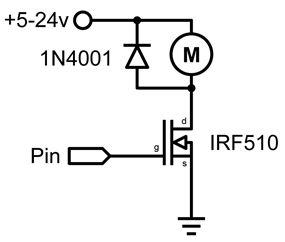
\includegraphics[width=120pt]{./Imagenes/Documentos/ArduinoNotebook_img03.png}
	\caption[Conexión salida de alta corriente de consumo]{Conexión salida de alta corriente de consumo}
\end{figure}

A veces es necesario controlar cargas de más de los 40 mA que es capaz de suministrar la tarjeta Arduino. En este caso se hace uso de un transistor MOSFET que puede alimentar cargas de mayor consumo de corriente. El siguiente ejemplo muestra como el transistor MOSFET conmuta 5 veces cada segundo.\\\\
\textbf{Nota}: El esquema muestra un motor con un diodo de protección por ser una carga inductiva. En los casos que las cargas no sean inductivas no será necesario colocar el diodo.
\begin{lstlisting}
int outPin = 5; // pin de salida para el MOSFET

void setup()
{
   pinMode(outPin, OUTPUT); // pin5 como salida
}

void loop()
{
   for (int i=0; i<=5; i++)     // repetir bucle 5 veces
   {
      digitalWrite(outPin, HIGH); // activa el MOSFET
      delay(250); // espera 1/4 segundo
      digitalWrite(outPin, LOW); // desactiva el MOSFET
      delay(250); // espera 1/4 segundo
   }
   delay(1000); // espera 1 segundo
}
\end{lstlisting}
\section{Salida analógica del tipo pwm}
PWM (modulación de impulsos en frecuencia)
\begin{figure}[!htp]
	\centering
	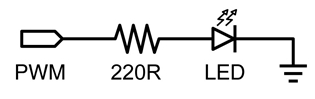
\includegraphics[width=120pt]{./Imagenes/Documentos/ArduinoNotebook_img04.png}
	\caption[Conexión salida analógica del tipo pwm]{Conexión salida analógica del tipo pwm}
\end{figure}


La Modulación por Anchura de Pulsos (PWM) es una forma de conseguir una “falsa” salida analógica. Esto podría ser utilizado para modificar el brillo de un LED o controlar un servo motor. El siguiente ejemplo hace que el LED se ilumine y se apague lentamente haciendo uso de dos bucles.
\begin{lstlisting}
int ledPin = 9; // pin PWM para el LED

void setup(){} // no es necesario configurar nada

void loop()
{
   for (int i=0; i<=255; i++) // el valor de i asciende
   {
      analogWrite(ledPin, i); // se escribe el valor de I en el PIN de salida del LED
      delay(100); // pauses for 100ms
   }
   for (int i=255; i>=0; i--) // el valor de I desciendei
   {
      analogWrite(ledPin, i); // se escribe el valor de ii
      delay(100); // pasusa durante 100ms
   }
}
\end{lstlisting}
\newpage{}
\section{Entrada con potenciómetro}
\begin{figure}[!htp]
	\centering
	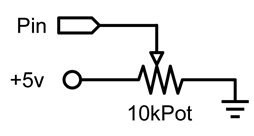
\includegraphics[width=120pt]{./Imagenes/Documentos/ArduinoNotebook_img05.png}
	\caption[Conexión entrada con potenciometro]{Conexión entrada con potenciometro}
\end{figure}

El uso de un potenciómetro y uno de los pines de entrada analógica-digital de Arduino (ADC) permite leer valores analógicos que se convertirán en valores dentro del rango de 0-1023. El siguiente ejemplo utiliza un potenciómetro para controlar un el tiempo de parpadeo de un LED.
\begin{lstlisting}
int potPin = 0; // pin entrada para potenciometro
int ledPin = 13;     // pin de salida para el LED

void setup()
{
   pinMode(ledPin, OUTPUT);     // declara ledPin como SALIDA
}

void loop()
{
   digitalWrite(ledPin, HIGH); // pone ledPin en on
   delay(analogRead(potPin)); // detiene la ejecucion un tiempo 'potPin'
   digitalWrite(ledPin, LOW); // pone ledPin en off
   delay(analogRead(potPin)); // detiene la ejecucion un tiempo 'potPin'
}
\end{lstlisting}
\newpage{}
\section{Entrada conectada a resistencia variable}

\begin{figure}[!htp]
	\centering
	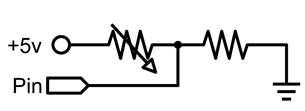
\includegraphics[width=120pt]{./Imagenes/Documentos/ArduinoNotebook_img06.png}
	\caption[Conexión entrada con resistencia variable]{Conexión entrada con resistencia variable}
\end{figure}
Las resistencias variables como los sensores de luz LCD, los termistores, sensores de esfuerzos, etc, se conectan a las entradas analógicas para recoger valores de parámetros físicos. Este ejemplo hace uso de una función para leer el valor analógico y establecer un tiempo de retardo. Este tiempo controla el brillo de un diodo LED conectado en la salida.
\begin{lstlisting}
int ledPin = 9; // Salida analogica PWM para conectar a LED
int analogPin = 0; // resistencia variable conectada a la entrada analogica pin 0

void setup(){}    // no es necesario configurar entradas y salidas

void loop()
{
   for (int i=0; i<=255; i++) // incremento de valor de i
   {
      analogWrite(ledPin, i); // configura el nivel brillo con el valor de i
      delay(delayVal()); // espera un tiempo en milisegundos
   }
   for (int i=255; i>=0; i--) // decrementa el valor de i
   {
      analogWrite(ledPin, i); // configura el nivel de brillo con el valor de i
      delay(delayVal()); // espera un tiempo en milisegundos
   }
}

int delayVal() // Metodo para recoger el tiempo de retardo
{
   int v; // crea una variable temporal (local)

   v    = analogRead(analogPin); // lee valor analogico
   v *= 2;     // convierte el valor leido de 0-1023 a 0-2046
   return v; // devuelve el valor v
}
\end{lstlisting}
\section{Salida conectada a servo}
\begin{figure}[!htp]
	\centering
	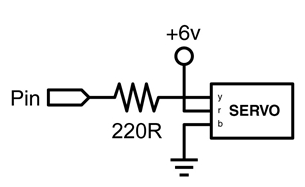
\includegraphics[width=90pt]{./Imagenes/Documentos/ArduinoNotebook_img07.png}
	\caption[Conexión salida conectada a servo]{Conexión salida conectada a servo}
\end{figure}

Los servos de los juguetes tienen un tipo de motor que se puede mover en un arco de 180 º y contienen la electrónica necesaria para ello. Todo lo que se necesita es un pulso enviado cada 20ms. Este ejemplo utiliza la función servoPulse para mover el servo de 10º a 170 º.
\begin{lstlisting}
int servoPin = 2; // servo conectado al pin digital 2
int myAngle; // angulo del servo de 0-180
int pulseWidth; // anchura del pulso para la funcion servoPulse

void setup()
{
   pinMode(servoPin, OUTPUT); // configura pin 2 como salida
}

void servoPulse(int servoPin, int myAngle)
{
   pulseWidth = (myAngle * 10) + 600; // determina retardo 
   digitalWrite(servoPin, HIGH); // activa el servo
   delayMicroseconds(pulseWidth); // pausa
   digitalWrite(servoPin, LOW); // desactiva el servo
   delay(20); // retardo de refresco
}

void loop()
{
// el servo inicia su recorrido en 10 y gira hasta 170
   for (myAngle=10; myAngle<=170; myAngle++)
   {
      servoPulse(servoPin, myAngle);
   }
// el servo vuelve desde 170 hasta 10
   for (myAngle=170; myAngle>=10; myAngle--)
   {
      servoPulse(servoPin, myAngle);
   }
}
\end{lstlisting}